\section{\label{sec:intro}Introduction}

%\begin{figure}
%  \centering
%  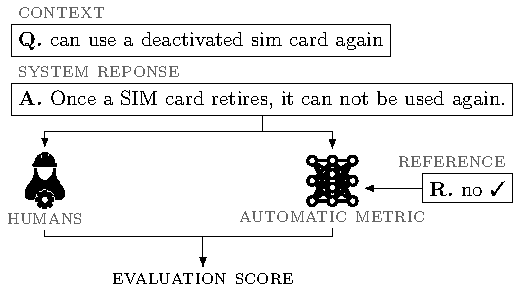
\includegraphics[width=\columnwidth]{figures/overview}
%  \caption{\label{fig:overview}
%  Current automatic metrics like ROUGE or BLEU systematically score system improvements that generate long, well-formed generations, such as the one shown above, poorly even though they score highly according to human evaluations.
%  In this work, we propose leverages the automatic metric to instead reduce the cost of a human evaluation without introducing bias.
%  }
%\end{figure}

% == 1. NLG evaluation is hard, human evaluation is expensive, automatic metrics are biased
In recent years, there has been an increasing interest in tasks that require generating natural language, including
  abstractive summarization~\citep{nallapati2016abstractive},
  open-response question answering~\citep{nguyen2016ms,kovcisky2017narrativeqa}, 
  % machine translation?
  image captioning~\citep{lin2014microsoft},
  and open-domain dialogue~\citep{lowe2017ubuntu}.
Unfortunately, the evaluation of these systems remains a thorny issue because of the diversity of possible correct responses.
As the gold standard of performing human evaluation is often too expensive,
there has been a large effort developing
automatic metrics such as BLEU~\citep{papineni02bleu}, ROUGE~\citep{lin2004rouge}, METEOR~\citep{lavie2009meteor,denkowski2014meteor} and CiDER~\citep{vedantam2015cider}.
However, these have shown to be biased, correlating poorly with human metrics across different datasets and systems~\citep{liu2016evaluate,novikova2017why}.
% PL: this is fine
%\ac{I'm worried this might be too strong a statement: no one has made explicit studies about bias, just that the correlation is low.}

% == 2. Key contribution: asking question and general intuition
Can we combine automatic metrics and human evaluation to obtain
an \emph{unbiased} estimate at \emph{lower cost} than human evaluation alone?
%We should hope that such a method can rely on the model to evaluate ``easy'' cases and on humans on ``hard'' cases~\reffig{overview}.
% PL: I don't think this is the intuition, because we're not doing importance sampling
%\ac{This intuition is not really borne out by our estimator and maybe not the figure we are looking for?}
In this paper,
we propose a simple estimator based on control variates~\citep{ripley2009stochastic},
where we average differences between human judgments and automatic metrics
rather than averaging the human judgments alone.
Provided the two are correlated,
our estimator will have lower variance and thus reduce cost.
%that automatically scales and shifts the automatic metric to best predict human judgment. % PL: not first-order bit
%As a result, this method is able to reduce the estimation problem from predicting the mean across each example in the dataset,
%which could vary a lot, to estimating just the mean difference between the automatic metric and human judgment.
%Thus, any automatic metric correlated with human judgments provably reduces the variance of our estimate and hence costs.

% == 3. Contribution 2: optimality and theoretical insight.
We prove that our estimator is \emph{optimal} in the sense
that no unbiased estimator using the same automatic metric can have lower variance.
%A theoretical analysis of our proposed estimator further shows that given an automatic metric with a fixed correlation it is \textit{optimal} in that no other unbiased estimator has a lower variance for the same amount of data.
We also analyze its data efficiency (equivalently, cost savings)---the factor reduction in number of human judgments needed to obtain the same accuracy versus naive human evaluation---and show that it depends solely on
two factors:
  (a) the annotator variance (which is a function of the human evaluation prompt) and
  (b) the correlation between human judgments and the automatic metric.
This factorization allows us to calculate typical and best-case data efficiencies and accordingly refine the evaluation prompt or automatic metric.

% == 4. Contribution 3: data and empirical results.
Finally, we evaluate our estimator on state-of-the-art systems from two tasks, summarization on the CNN/Daily Mail dataset~\citep{hermann2015read,nallapati2016abstractive}
and open-response question answering on the MS MARCOv1.0 dataset~\citep{nguyen2016ms}.
To study our estimators offline,
we preemptively collected 10,000 human judgments which cover several tasks and systems.\footnote{%
An anonymized version of this data and the annotation interfaces used can be found at \url{https://bit.ly/price-of-debiasing}.}
As predicted by the theory, we find that the data efficiency depends not only on the correlation between the human and automatic metrics,
but also on the evaluation prompt.
If the automatic metric had perfect correlation, our data efficiency would be around 3, while
  if we had noiseless human judgments, our data efficiency would be about 1.5.
In reality, the reduction in cost we obtained was only about 10\%,
suggesting that improvements in both automatic metric and evaluation prompt are needed.
As one case study in improving the latter, we show that, when compared to a Likert survey, measuring the amount of post-editing needed to fix a generated sentence
reduced the annotator variance by three-fold.

%We find that the human evaluation prompt strongly affects inter-annotator variance:
%for example, evaluating language quality using a Likert survey can have almost twice as much variance as measuring the average edit rate.
%In practice, we find that existing automatic metrics lead to only a \ac{10\%} reduction in costs for both of these tasks.
%Using the inter-annotator variance we measure, we find that the best-case cost savings are only about 3x for both tasks, suggesting that the limiting factor in reducing the costs of human evaluation is developing better annotation interfaces as opposed to better evaluation models. \ac{This last sentence is sketch. Technically, even with 0 annotation error, a model with a correlation of $0.8$ will still have a data efficiency of less than $3$.}
%\ac{Alternate, more accurate ending:}
%Using our measurements of inter-annotator variance, we find that the best-case cost savings are only about 3x for both tasks,
%highlighting the importance of developing good annotation interfaces in addition to improving our automatic metrics.
%Given these upper limits to how much we can scale human evaluation,
%we conclude that, at present, we must pick between an unbiased evaluation that is expensive and a biased one that is cheap.
%That said, even in the best case, in order for automatic metrics to reduce costs by more than a factor of $3$, we need to develop automatic metrics with a correlation of at least $0.8$, leading us to 

%\ac{Not sure where this should go, but I want to mention it somewhere.}

% == 5. Conclusions: recommendations and sharing data.
%Having a reliable evaluation measure that remains unbiased with variations in systems is incredibly vital to our ability to improve the state of the art.
%In summary, this paper provides an optimal approach to combining an automatic metric with human evaluation to reduce the costs of unbiased evaluation.
% How to combine automatic and human?
% In this paper, we propose turning the standard approach of evaluation on its head \stm{``on its head'' seems too hyperbolic}, and instead of looking for an automatic evaluation metric with high human correlation that we hope generalizes across inputs, we believe any evaluation metric we use should meet the standard of unbiasedness.
% This of course raises the concern of cost: we look instead to find ways to incorporate potentially noisy models within our estimation framework to reduce costs while still guaranteeing performance.
% 
% % Provide an intuitive example of how this approach would work.
% For example, if we were predicting language quality, we intuitively know that .
% 
% In this paper, we propose simple estimators that are able to incorporate either the model's \pl{surrogate} output or its reports of confidence \stm{how are we using the reports of confidence?}.
% While simple, we show that these estimators are in fact \textit{optimal}: no other estimator can have less variance while still being an unbiased estimator.
% These estimators allow us to predict data savings through the use of our framework using simple measurable properties of our task: annotator agreement, model correlation and model calibration.
% Thus, the framework guides the practitioner to incrementally improve X and Y.
% \pl{should describe at a high-level what the estimator is doing}
% \pl{say: (i) optimal, (ii) identify factors for improvement over naive human evaluation
% (I think you might say this but I can't tell)
% }
% 
% In addition to our theoretical contribution, we have collected datasets with annotations of several systems for four different subjective evaluation tasks: language quality evaluation (based on the CNN/Daily Mail summarization task), open-domain question answering (based on MSMarco), dialogue (based on the Twitter dataset and a negotiation task) and image captioning (based on MSCOCO).
% For some tasks, such as question answering, which has high annotator agreement, we find that our framework is able to significantly \pl{is this significant?} reduce the amount of data that needs to be collected by a factor of $1.5$. 
% On the other hand, for tasks like language quality evaluation, we are able to show that as defined, standard annotation practices limit the ability for data savings with any method.  
% 
% In summary, our contributions are:
% 1. an optimal unbiased estimator to evaluate natural language generation using on-demand evaluation and a model, 
% 2. datasets with annotations and systems for several tasks that allow us to develop better evaluation methods,
% 3. an instantiation of the framework to measure possible gains for each of these tasks.
% 
% We make both our data and our annotation interfaces available. 
% We release a software library that allows users to take advantage of our research through a simple API call and receive human evaluation for cheap.
% As of writing this article, only n out of the previous m publications in the ACL anthology included a human evaluation, partly because of cost and partly because of several factors involved.
% We hope that the framework presented here will make it easier for the community to report reliable human evaluation metrics in our papers.
